\chapter{Testing and Results}

Testing was carried out at four levels: unit tests of the agent and backend, user
interface tests of the dashboard, security tests, and an experimental evaluation of
detection quality and performance. The evaluation uses three kinds of data: the
synthetic test set, real-world data (BETH and the Kubernetes escape recording), and a
live attack simulation in the minikube cluster.

\section{Unit Testing}

Unit tests are written with \textbf{pytest}. The backend tests run against a temporary
MongoDB container. All 19 tests pass (Table~\ref{tab:unittests}).

\begin{longtable}{>{\ttfamily\footnotesize}p{6.2cm} >{\raggedright\arraybackslash}p{5.6cm} c}
\caption{Unit tests and results}\label{tab:unittests}\\
\toprule
\normalfont\textbf{Test} & \textbf{What is verified} & \textbf{Result} \\
\midrule
\endfirsthead
\toprule
\normalfont\textbf{Test} & \textbf{What is verified} & \textbf{Result} \\
\midrule
\endhead
\multicolumn{3}{l}{\textit{Agent (services/ebpf-agent/tests) -- 13 tests}} \\
test\_\allowbreak{}normalise\_\allowbreak{}exec\_\allowbreak{}and\_\allowbreak{}connect & Kernel records become pipeline events & Pass \\
test\_\allowbreak{}runc\_\allowbreak{}is\_\allowbreak{}not\_\allowbreak{}netcat & v0 bug: \texttt{runc} no longer matches ``nc'' & Pass \\
test\_\allowbreak{}dev\_\allowbreak{}substring\_\allowbreak{}is\_\allowbreak{}not\_\allowbreak{}suspicious\_\allowbreak{}dir & v0 bug: \texttt{/dev} is not a temp dir & Pass \\
test\_\allowbreak{}features\_\allowbreak{}use\_\allowbreak{}full\_\allowbreak{}argv & Features use all arguments & Pass \\
test\_\allowbreak{}wait\_\allowbreak{}for\_\allowbreak{}is\_\allowbreak{}not\_\allowbreak{}reverse\_\allowbreak{}shell & \texttt{nc -z} wait loops not flagged & Pass \\
test\_\allowbreak{}base64\_\allowbreak{}blob\_\allowbreak{}vs\_\allowbreak{}long\_\allowbreak{}path & Base64 detection vs.\ long paths & Pass \\
test\_\allowbreak{}rules\_\allowbreak{}fire\_\allowbreak{}on\_\allowbreak{}attacks & Rules match attack events & Pass \\
test\_\allowbreak{}rules\_\allowbreak{}quiet\_\allowbreak{}on\_\allowbreak{}platform\_\allowbreak{}behaviour & Platform exemptions work & Pass \\
test\_\allowbreak{}behaviour\_\allowbreak{}tracker\_\allowbreak{}window\_\allowbreak{}and\_\allowbreak{}new\_\allowbreak{}binary & 60 s window and new-binary flag & Pass \\
test\_\allowbreak{}cgroup\_\allowbreak{}regexes\_\allowbreak{}and\_\allowbreak{}workloads & Pod UID, container ID, workload & Pass \\
test\_\allowbreak{}model\_\allowbreak{}separates\_\allowbreak{}attacks\_\allowbreak{}from\_\allowbreak{}benign & Trained model ranks attacks higher & Pass \\
test\_\allowbreak{}assess\_\allowbreak{}produces\_\allowbreak{}alert\_\allowbreak{}with\_\allowbreak{}mitre & Decision has severity and MITRE & Pass \\
test\_\allowbreak{}platform\_\allowbreak{}namespace\_\allowbreak{}needs\_\allowbreak{}high\_\allowbreak{}confidence & 0.75 threshold in platform namespaces & Pass \\
\midrule
\multicolumn{3}{l}{\textit{Backend (services/backend/tests) -- 6 tests}} \\
test\_\allowbreak{}login\_\allowbreak{}rejects\_\allowbreak{}bad\_\allowbreak{}password & Wrong password returns 401 & Pass \\
test\_\allowbreak{}dashboard\_\allowbreak{}requires\_\allowbreak{}jwt & API rejects requests without JWT & Pass \\
test\_\allowbreak{}ingest\_\allowbreak{}requires\_\allowbreak{}agent\_\allowbreak{}token & Ingest rejects missing / wrong token & Pass \\
test\_\allowbreak{}ingest\_\allowbreak{}events\_\allowbreak{}and\_\allowbreak{}dedup\_\allowbreak{}alerts & Events stored, alerts merged & Pass \\
test\_\allowbreak{}alert\_\allowbreak{}lifecycle & Open $\rightarrow$ acknowledged $\rightarrow$ resolved & Pass \\
test\_\allowbreak{}stats\_\allowbreak{}agents\_\allowbreak{}evaluation & Statistics and evaluation endpoints & Pass \\
\bottomrule
\end{longtable}

\section{User Interface Testing}

The dashboard was tested in a real browser with \textbf{Playwright} (Chrome). The test
script logs in with the administrator account, opens every page (Overview, Alerts,
Events, Evaluation), opens an alert's detail panel, applies the ``suspicious'' filter on
the Events page and takes the screenshots shown in Chapter~7. All pages loaded and
displayed live data. The test exposed one layout defect: in the attack-simulation table
of the Evaluation page the result column is too narrow, so only the first rows are
visible without scrolling; this is listed under future work.

\section{Security Testing}

\begin{itemize}
    \item \textbf{Authentication:} dashboard endpoints return 401 without a valid JWT; the
          ingest endpoints reject requests without the agent token (verified by unit tests).
    \item \textbf{Password storage:} the admin password is stored as a bcrypt hash; the
          plain password exists only in the Kubernetes Secret.
    \item \textbf{Secrets:} all credentials are random values generated at deployment, not
          hard-coded in the source code or images.
    \item \textbf{Least privilege:} the agent's ClusterRole allows only reading pods; the
          backend and frontend run without privileges. Only the agent is privileged, which
          is required to load eBPF programs.
    \item \textbf{Robustness:} malformed events and failing rules are skipped without
          stopping the sensor; kernel drops are counted and shown on the dashboard.
\end{itemize}

\section{Evaluation Metrics}

With TP, TN, FP and FN denoting true positives, true negatives, false positives and
false negatives (malicious = positive class), the following metrics are reported:
\begin{align}
\mathrm{Accuracy} &= \frac{TP + TN}{TP + TN + FP + FN} \\
\mathrm{Precision} &= \frac{TP}{TP + FP} \\
\mathrm{Recall\ (detection\ rate)} &= \frac{TP}{TP + FN} \\
\mathrm{FPR} &= \frac{FP}{FP + TN} \\
F_1 &= 2 \cdot \frac{\mathrm{Precision} \cdot \mathrm{Recall}}{\mathrm{Precision} + \mathrm{Recall}}
\end{align}
ROC-AUC is the area under the curve of recall against FPR over all thresholds; it
measures how well the model \emph{ranks} malicious events above benign ones,
independently of the chosen threshold. For an IDS the false-positive rate matters as
much as recall: on a busy node even 1\% false positives produce many alerts per hour.

\section{Results on the Synthetic Data (Deployed Model)}

The model deployed in the cluster (\texttt{rf-20261107-161508}) was trained on the
40,000-row synthetic dataset. Table~\ref{tab:offline} shows its results on a stratified
20\% hold-out and on harder subsets, compared with the Isolation Forest baseline of the
v0 prototype; Figure~\ref{fig:cm-holdout} shows the hold-out confusion matrix.

\begin{table}[H]
\centering
\caption{Offline results of the deployed model (synthetic data, threshold 0.5)}
\label{tab:offline}
\small
\begin{tabular}{lrrrrrr}
\toprule
\textbf{Test set} & \textbf{Samples} & \textbf{Recall} & \textbf{FPR} & \textbf{Precision} & \textbf{F1} & \textbf{AUC} \\
\midrule
Hold-out (stratified 20\%) & 8,000 & 98.7\% & 0.18\% & 99.5\% & 0.9905 & 0.9997 \\
Edge cases only            & 4,930 & 98.1\% & 0.29\% & 99.0\% & 0.9853 & 0.9995 \\
Non-edge cases             & 3,070 & 99.3\% & 0.00\% & 100.0\% & 0.9967 & 0.9999 \\
Unseen template families   & 6,138 & 90.4\% & 15.89\% & 76.2\% & 0.8269 & 0.9621 \\
\midrule
Baseline: Isolation Forest & 8,000 & 12.0\% & 1.28\% & 75.7\% & 0.2072 & 0.5536 \\
\bottomrule
\end{tabular}
\end{table}

\begin{figure}[H]
\centering
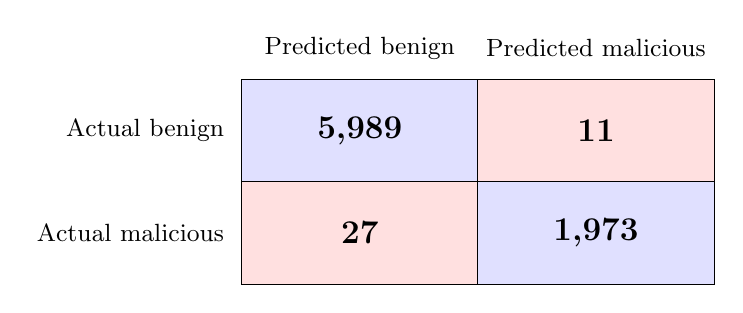
\begin{tikzpicture}[cell/.style={draw, minimum width=3cm, minimum height=1.3cm, font=\large\bfseries}]
  \node[cell, fill=blue!12] at (0,0) {5,989};
  \node[cell, fill=red!12] at (3,0) {11};
  \node[cell, fill=red!12] at (0,-1.3) {27};
  \node[cell, fill=blue!12] at (3,-1.3) {1,973};
  \node[font=\small] at (0,1.05) {Predicted benign};
  \node[font=\small] at (3,1.05) {Predicted malicious};
  \node[font=\small, anchor=east] at (-1.6,0) {Actual benign};
  \node[font=\small, anchor=east] at (-1.6,-1.3) {Actual malicious};
\end{tikzpicture}
\caption{Confusion matrix of the deployed model on the synthetic hold-out set}
\label{fig:cm-holdout}
\end{figure}

\textbf{Observations.} Accuracy on the hold-out set is 99.52\% and five-fold
cross-validation gives $F_1 = 0.9903 \pm 0.0006$. The Random Forest detects eight
times more attacks than the Isolation Forest baseline at a lower false-positive rate.
The ``unseen template families'' row trains without whole families of commands and
tests on them; its recall of 90.4\% at 15.9\% FPR is the more realistic estimate of
generalisation, and closing this gap is the job of the rule layer. The most important
features are the behaviour-window counters (sensitive opens, shell count, execution
count, new binary), command-line length and entropy, and whether the parent is a
server process. Inference takes 0.04~ms per event in batches of 256.

\section{Results on the Final Test Set}

A second model (\texttt{rf-20261122-223113}) was trained with exactly the same method
on the final \texttt{train.csv} (synthetic data plus 25,000 real benign BETH events) and
tested once on \texttt{test.csv} (Section~4.5). No parameter or threshold was tuned on
the test set.

\subsection{Validation on the Training Data}

\begin{table}[H]
\centering
\caption{Validation of the final model on \texttt{train.csv}}
\label{tab:finalval}
\small
\begin{tabular}{lrrrrr}
\toprule
\textbf{Check} & \textbf{Accuracy} & \textbf{Precision} & \textbf{Recall} & \textbf{FPR} & \textbf{F1} \\
\midrule
Stratified 20\% hold-out (13,000)   & 0.9975 & 0.9945 & 0.9895 & 0.10\% & 0.9920 \\
Edge cases only (4,906)             & 0.9945 & 0.9906 & 0.9842 & 0.26\% & 0.9874 \\
Unseen template families (7,711)    & 0.9684 & 0.9894 & 0.9105 & 0.46\% & 0.9483 \\
5-fold cross-validation             & --     & --     & 0.9877 & 0.10\% & 0.9912 \\
Baseline: Isolation Forest          & 0.8679 & 0.7737 & 0.2000 & 1.06\% & 0.3178 \\
\bottomrule
\end{tabular}
\end{table}

Adding real benign data reduced the false-positive rate on unseen template families
from 15.89\% to 0.46\%.

\subsection{Binary Results per Test Source}

\begin{table}[H]
\centering
\caption{Final model on \texttt{test.csv} (ML only, threshold 0.5)}
\label{tab:finaltest}
\scriptsize
\setlength{\tabcolsep}{3pt}
\begin{tabular}{lrrrrrrrrrr}
\toprule
\textbf{Source} & \textbf{Samples} & \textbf{Acc.} & \textbf{Prec.} & \textbf{Recall} & \textbf{FPR} & \textbf{F1} & \textbf{AUC} & \textbf{FP} & \textbf{FN} & \textbf{TP} \\
\midrule
Synthetic        & 20,000  & 0.9939 & 0.9986 & 0.9860 & 0.09\% & \textbf{0.9923} & 0.9998 & 11 & 112 & 7,888 \\
BETH (real)      & 262,825 & 0.4427 & 0.9988 & 0.0056 & 0.00\% & \textbf{0.0112} & 0.9995 & 1 & 146,479 & 829 \\
K8s escape       & 25      & 0.7200 & 0.5000 & 0.1429 & 5.56\% & \textbf{0.2222} & 0.6746 & 1 & 6 & 1 \\
\midrule
All (ML only)    & 282,850 & 0.4817 & 0.9985 & 0.0561 & 0.01\% & 0.1063 & 0.9991 & 13 & 146,597 & 8,718 \\
All (ML + rules) & 282,850 & 0.4794 & 0.9230 & 0.0566 & 0.57\% & 0.1066 & -- & 733 & 146,527 & 8,788 \\
\bottomrule
\end{tabular}
\end{table}

\begin{figure}[H]
\centering
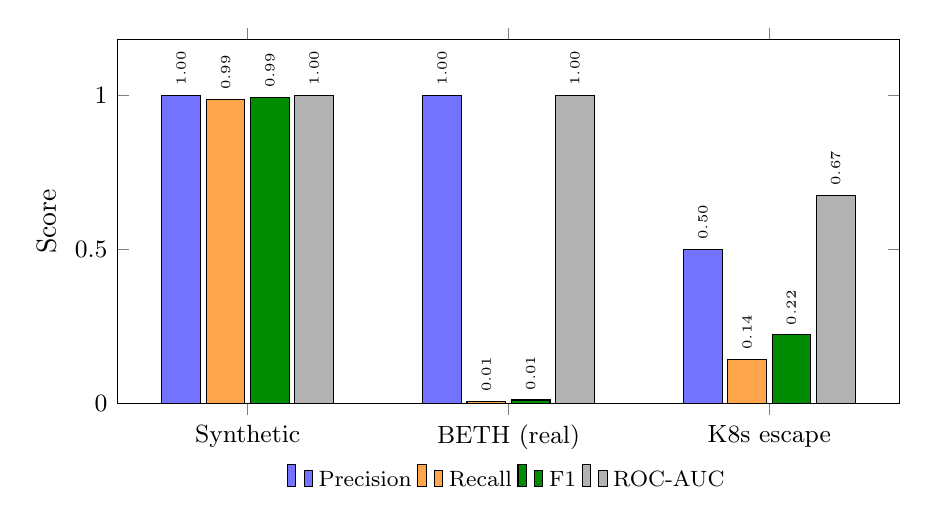
\begin{tikzpicture}
\begin{axis}[
    ybar, bar width=14pt, width=0.95\textwidth, height=6.2cm,
    ymin=0, ymax=1.18, ylabel={Score},
    symbolic x coords={Synthetic, BETH (real), K8s escape},
    xtick=data, enlarge x limits=0.25,
    legend style={at={(0.5,-0.15)}, anchor=north, legend columns=-1, font=\footnotesize, draw=none},
    nodes near coords, nodes near coords style={/pgf/number format/fixed, /pgf/number format/fixed zerofill, /pgf/number format/precision=2},
    every node near coord/.append style={font=\tiny, rotate=90, anchor=west},
    tick label style={font=\small}]
  \addplot[fill=blue!55] coordinates {(Synthetic,0.9986) (BETH (real),0.9988) (K8s escape,0.5)};
  \addplot[fill=orange!70] coordinates {(Synthetic,0.986) (BETH (real),0.0056) (K8s escape,0.1429)};
  \addplot[fill=green!55!black] coordinates {(Synthetic,0.9923) (BETH (real),0.0112) (K8s escape,0.2222)};
  \addplot[fill=gray!60] coordinates {(Synthetic,0.9998) (BETH (real),0.9995) (K8s escape,0.6746)};
  \legend{Precision, Recall, F1, ROC-AUC}
\end{axis}
\end{tikzpicture}
\caption{Precision, recall, F1 and ROC-AUC of the final model per test source}
\label{fig:persource}
\end{figure}

\subsection{Multi-Class Results}

On all test rows whose true category is known (synthetic, Kubernetes escape and BETH
benign events), the model reaches a multi-class accuracy of 99.68\%, a macro-averaged
F1 of 0.9554 and a weighted F1 of 0.9968 (Table~\ref{tab:multiclass}).

\begin{table}[H]
\centering
\caption{Per-class results of the final model on \texttt{test.csv}}
\label{tab:multiclass}
\small
\begin{tabular}{lrrrr}
\toprule
\textbf{Class} & \textbf{Precision} & \textbf{Recall} & \textbf{F1} & \textbf{Support} \\
\midrule
Benign               & 0.9981 & 1.0000 & 0.9991 & 127,535 \\
Container escape     & 0.9975 & 0.9736 & 0.9854 & 833 \\
Credential access    & 0.9987 & 0.9544 & 0.9761 & 812 \\
Crypto-miner         & 0.9972 & 0.9273 & 0.9610 & 757 \\
Defense evasion      & 0.9983 & 0.9190 & 0.9570 & 630 \\
Discovery            & 0.9344 & 0.9712 & 0.9525 & 939 \\
Dropper / payload    & 0.9701 & 0.9719 & 0.9710 & 1,102 \\
Lateral movement     & 0.9590 & 0.7524 & 0.8432 & 311 \\
Privilege escalation & 0.9205 & 0.9399 & 0.9301 & 949 \\
Reverse shell        & 0.9994 & 0.9582 & 0.9783 & 1,674 \\
\midrule
Macro average        & 0.9773 & 0.9368 & 0.9554 & \\
\bottomrule
\end{tabular}
\end{table}

The weakest class is lateral movement, which is often confused with discovery (54 of
311 events) because both consist of connections to internal services.

\subsection{Comparison with the Deployed Model}

\begin{table}[H]
\centering
\caption{Deployed model vs.\ final model on \texttt{test.csv} (ML only, threshold 0.5)}
\label{tab:compare}
\small
\begin{tabular}{lcc}
\toprule
\textbf{Test source} & \textbf{Deployed model} & \textbf{Final model} \\
 & F1 / Recall / FP & F1 / Recall / FP \\
\midrule
Synthetic          & 0.9921 / 0.9862 / 15  & 0.9923 / 0.9860 / 11 \\
BETH (real)        & 0.6869 / 0.5248 / 481 & 0.0112 / 0.0056 / 1 \\
Kubernetes escape  & 0.2222 / 0.1429 / 1   & 0.2222 / 0.1429 / 1 \\
\bottomrule
\end{tabular}
\end{table}

\subsection{Analysis of the Real-World Results}

\begin{itemize}
    \item \textbf{False positives almost eliminated.} Real benign host activity in the
          training data (\texttt{ps} reading \texttt{/proc}, \texttt{sshd}, systemd) cut
          the false positives on the BETH test hosts from 481 to 1.
    \item \textbf{Recall on BETH collapsed at the 0.5 threshold.} 144,801 of the 147,308
          malicious BETH events come from one SSH-scanning bot. Benign \texttt{sshd}
          connections to port 22 in the new training data lowered the scanner's score to
          about 0.47, just below the threshold. The ranking is still excellent (ROC-AUC
          0.9995): the scanner is scored above almost all benign events, but not above
          0.5. The root cause is a training gap: no synthetic attack contains more than 12
          distinct destinations in its window, whereas the scanner contacts about 3,200.
    \item \textbf{Threshold.} At thresholds of 0.2--0.3 the F1 on the whole test set would
          exceed 0.99. This was deliberately \emph{not} used, because choosing the
          threshold on the test set would make the test result meaningless, and the
          improvement is caused by a single cluster of scanner events.
    \item \textbf{Other BETH attacks} (about 2,500 events) are partly label noise (BETH
          labels routine commands of the attacker's session as evil) and partly real
          misses, such as \texttt{wget} from a raw IP address (score 0.49) and
          \texttt{modprobe msr} (0.29).
    \item \textbf{Kubernetes escape.} Only the \texttt{nsenter --target 1} step is flagged
          (rule R014 and ML); the follow-up actions are missed. The recording contains only
          process executions, whereas the live sensor would also observe the
          \texttt{open} of \texttt{/root/.ssh/authorized\_keys} and the \texttt{mount}
          system call, which the rules target. The incident as a whole is detected.
\end{itemize}
These results confirm the observation of Sommer and Paxson~\cite{sommer2010}: excellent
in-distribution results do not guarantee real-world performance. For this reason the
deployed model was \emph{not} replaced by the final model.

\section{Live Cluster Evaluation}

The script \texttt{evaluation/run\_live\_eval.py} runs 20 harmless attack re-enactments
and 15 benign look-alike commands with \texttt{kubectl exec} inside the test workload
\texttt{ids-demo/shop-web} and checks which of them produce an alert. It then measures
execution overhead by running 2,000 fork+exec operations with and without the agent.
Table~\ref{tab:live} summarises the run of 22 November 2026; Table~\ref{tab:scenarios}
lists every scenario.

\begin{table}[H]
\centering
\caption{Live evaluation in minikube}
\label{tab:live}
\small
\begin{tabular}{ll}
\toprule
\textbf{Metric} & \textbf{Result} \\
\midrule
Attack scenarios detected & \textbf{20 / 20 (100\%)} \\
Benign scenarios flagged (false positives) & 4 / 15 (26.7\%) \\
Detection latency (kernel event $\rightarrow$ verdict) & average \textbf{123 ms}, p95 269 ms \\
Kernel events dropped & 0 \\
Agent CPU (normal load) & 3.5\% of one core \\
Agent memory & 198 MB (agent 189 MB + loader 9 MB) \\
Event throughput during the run & 23.5 events/s \\
Execution overhead (2,000 $\times$ fork+exec) & +21.4\% (0.634 s vs.\ 0.522 s) \\
\bottomrule
\end{tabular}
\end{table}

{\small
\begin{longtable}{>{\raggedright\arraybackslash}p{4.4cm} l l l >{\raggedright\arraybackslash}p{3.2cm}}
\caption{Live attack and benign scenarios}\label{tab:scenarios}\\
\toprule
\textbf{Scenario} & \textbf{Kind} & \textbf{Result} & \textbf{Sev.} & \textbf{Latency / rules} \\
\midrule
\endfirsthead
\toprule
\textbf{Scenario} & \textbf{Kind} & \textbf{Result} & \textbf{Sev.} & \textbf{Latency / rules} \\
\midrule
\endhead
Bash reverse shell & attack & detected & High & 109 ms, R001, R002 \\
Netcat reverse shell & attack & detected & High & 177 ms, R001, R002 \\
Python reverse shell & attack & detected & High & 32 ms, R001, R002 \\
Download piped to shell & attack & detected & High & 58 ms, R006 \\
Hidden binary run from /tmp & attack & detected & High & 215 ms, R007 \\
Crypto-miner process & attack & detected & High & 210 ms, R005 \\
Miner connecting to pool & attack & detected & High & 25 ms, R005, R007 \\
Service-account token theft & attack & detected & High & 150 ms, R003 \\
Password database read & attack & detected & High & 37 ms, R004 \\
Cloud metadata query & attack & detected & High & 152 ms, R015 \\
SUID shell backdoor & attack & detected & High & 36 ms, R010 \\
Cron persistence & attack & detected & High & 155 ms, R006, R016 \\
nsenter into host namespaces & attack & detected & High & 29 ms, R014 \\
User-namespace unshare & attack & detected & High & 140 ms, R014 \\
Docker socket access & attack & detected & High & 269 ms, R014 \\
Kubelet API access & attack & detected & High & 131 ms, R017 \\
Internal port scan & attack & detected & High & 36 ms, R018 \\
Container recon & attack & detected & Low & 235 ms, ML only \\
Fileless memfd payload & attack & detected & High & 73 ms, R012 \\
History / log wiping & attack & detected & Medium & 191 ms, R013 \\
\midrule
List application files & benign & clean & -- & -- \\
Read hostname & benign & clean & -- & -- \\
Python one-liner & benign & clean & -- & -- \\
Local health check (curl) & benign & false positive & Medium & ML only \\
Wait-for dependency (nc -z) & benign & false positive & Medium & ML only \\
Port check via /dev/tcp & benign & false positive & Medium & ML only \\
Process listing & benign & clean & -- & -- \\
Decode base64 config & benign & clean & -- & -- \\
pip version & benign & clean & -- & -- \\
Find python files & benign & clean & -- & -- \\
Backup app directory & benign & clean & -- & -- \\
Pretty-print JSON config & benign & clean & -- & -- \\
Check environment variable & benign & clean & -- & -- \\
Disk usage & benign & clean & -- & -- \\
Fetch own API (wget) & benign & false positive & Medium & ML only \\
\bottomrule
\end{longtable}
}

\textbf{Observations.} Every attack was detected, 18 of 20 with High severity and
most of them by both a rule and the model. All four false positives are ML-only
verdicts for network checks (\texttt{curl}, \texttt{nc -z}, \texttt{/dev/tcp},
\texttt{wget} to localhost) typed in an interactive \texttt{kubectl exec} shell, which
the model associates with attacker sessions; no rule fired for them. The same checks
run from an entrypoint or a probe look different in the behaviour window and are not
flagged in the training data. Detection latency is well below one second, no kernel
events were lost and the agent's CPU and memory use are small. The execution overhead
of 21\% is a worst-case micro-benchmark in which every one of 2,000 back-to-back
executions is captured and scored in Python; at the normal event rate of a few events
per second the overhead is negligible.

\section{Summary of Results}

\begin{itemize}
    \item On synthetic data the model reaches \textbf{F1 = 0.992} with a false-positive
          rate below 0.2\%, eight times the detection rate of the Isolation Forest
          baseline.
    \item In the live cluster the complete system (eBPF sensor, ML and rules) detected
          \textbf{20 of 20 attacks} with an average latency of \textbf{123 ms}, 3.5\% CPU
          and about 200 MB of memory.
    \item On real-world data precision stays very high, but recall shows that the
          synthetic attack examples do not cover real attacker behaviour such as mass SSH
          scanning; improving the training data is the most important next step.
\end{itemize}
